\begin{exercises}
    \subsection{Bài tập}

    \begin{questions}[series=SGK]
        \item Một nhóm học sinh đã khảo sát ý kiến về ý thức giữ gìn vệ sinh công cộng của các bạn trong trường với các mức đánh giá Tốt, Khá, Trung bình, Kém và thu được kết quả như sau:

        Tốt, Trung bình, Tốt, Trung bình, Khá, Tốt, Khá, Tốt, Tốt, Khá, Trung bình, Kém, Khá, Tốt, Khá, Tốt, Trung bình, Khá, Tốt, Tốt, Tốt, Khá, Kém, Trung bình, Tốt, Khá, Tốt, Khá, Tốt, Khá, Khá.

        \begin{questions}
            \item Lập bảng tần số cho dãy dữ liệu trên.

            \answerline
            \answerline

            \item Từ bảng tần số, hãy cho biết mức đánh giá nào chiếm ưu thế nhất. Vì sao?

            \answerline
        \end{questions}

        \item Cho biểu đồ tranh biểu diễn số lượng học sinh trong lớp đăng kí tham gia các câu lạc bộ của trường như sau:

        \begin{center}
        \begin{tikzpicture}
            \draw (0,0)--(15,0)--(15,2.5)--(0,2.5)--cycle;
            \draw (0,1.6)--(15,1.6);
            \draw (5,0)--(5,2.5);
            \draw (10,0)--(10,2.5);
            \node[font=\bfseries] at (2.5,2.05) {Câu lạc bộ võ thuật};
            \node[font=\bfseries] at (7.5,2.05) {Câu lạc bộ tiếng Anh};
            \node[font=\bfseries] at (12.5,2.05) {Câu lạc bộ nghệ thuật};

            \foreach \x in {1.0,1.65,2.3,2.95,3.6,4.25} {
                \draw (\x,1.05) circle (0.10);
                \draw (\x,0.95)--(\x,0.55);
                \draw (\x-0.14,0.80)--(\x+0.14,0.80);
                \draw (\x,0.55)--(\x-0.13,0.30);
                \draw (\x,0.55)--(\x+0.13,0.30);
            }
            \foreach \x in {5.45,6.05,6.65,7.25,7.85,8.45,9.05,9.65} {
                \draw (\x,1.05) circle (0.10);
                \draw (\x,0.95)--(\x,0.55);
                \draw (\x-0.14,0.80)--(\x+0.14,0.80);
                \draw (\x,0.55)--(\x-0.13,0.30);
                \draw (\x,0.55)--(\x+0.13,0.30);
            }
            \foreach \x in {11.1,11.8,12.5,13.2,13.9} {
                \draw (\x,1.05) circle (0.10);
                \draw (\x,0.95)--(\x,0.55);
                \draw (\x-0.14,0.80)--(\x+0.14,0.80);
                \draw (\x,0.55)--(\x-0.13,0.30);
                \draw (\x,0.55)--(\x+0.13,0.30);
            }
        \end{tikzpicture}

        \textit{(Mỗi }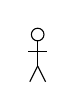
\begin{tikzpicture}[baseline=-0.4ex]
            \draw (0,0.25) circle (0.08);
            \draw (0,0.17)--(0,-0.15);
            \draw (-0.12,0.04)--(0.12,0.04);
            \draw (0,-0.15)--(-0.10,-0.35);
            \draw (0,-0.15)--(0.10,-0.35);
        \end{tikzpicture}\textit{ biểu diễn cho 1 học sinh)}
        \end{center}

        Lập bảng tần số cho dữ liệu được biểu diễn trong biểu đồ tranh trên.

        \answerline
        \answerline

        \item Biểu đồ Hình 7.7 cho biết số ngày sử dụng phương tiện đến trường của bạn Mai trong tháng Chín. Lập bảng tần số cho dữ liệu được biểu diễn trên biểu đồ.

        \begin{center}
        \begin{tikzpicture}[x=2cm,y=0.28cm]
            \foreach \y in {0,2,4,6,8,10,12,14,16} {
                \draw[base200] (0,\y)--(3.8,\y);
                \node[left] at (0,\y) {\y};
            }
            \draw[->] (0,0)--(4,0);
            \draw[->] (0,0)--(0,17);
            \foreach \x/\lab in {0.7/Xe buýt,1.9/Xe máy,3.1/Xe đạp} {
                \node[below,align=center] at (\x,0) {\lab};
            }
            \foreach \x/\h in {0.7/9,1.9/5,3.1/8} {
                \fill[base700] (\x-0.25,0) rectangle (\x+0.25,\h);
                \node[above] at (\x,\h) {\h};
            }
            \node[font=\bfseries] at (1.9,19) {Phương tiện đến trường của Mai};
            \node[below] at (1.9,-2.4) {Phương tiện đến trường};
            \node[rotate=90] at (-0.75,8.5) {Số ngày};
        \end{tikzpicture}

        \textit{Hình 7.7}
        \end{center}

        \answerline
        \answerline

        \item Người ta thống kê các loại ô tô chạy qua một trạm thu phí trong 1 giờ và vẽ được biểu đồ tần số như Hình 7.8.

        \begin{center}
        \begin{tikzpicture}[x=1.9cm,y=0.28cm]
            \foreach \y in {0,5,10,15} {
                \draw[base200] (0,\y)--(4.8,\y);
                \node[left] at (0,\y) {\y};
            }
            \draw[->] (0,0)--(5,0);
            \draw[->] (0,0)--(0,16);
            \foreach \x/\lab in {0.6/{Xe\\4 chỗ},1.7/{Xe\\7 chỗ},2.8/{Xe\\9 chỗ},4.0/{Xe 16 chỗ\\trở lên}} {
                \node[below,align=center] at (\x,0) {\lab};
            }
            \draw[base700,thick] (0.6,9)--(1.7,14)--(2.8,5)--(4.0,3);
            \foreach \x/\h in {0.6/9,1.7/14,2.8/5,4.0/3} {
                \fill[base700] (\x,\h) circle (2pt);
                \node[above right] at (\x,\h) {\h};
            }
            \node[font=\bfseries] at (2.4,18) {Số lượng các loại ô tô};
            \node[below] at (2.4,-4.1) {Loại xe};
            \node[rotate=90] at (-0.8,8) {Số xe};
        \end{tikzpicture}

        \textit{Hình 7.8}
        \end{center}

        \begin{questions}
            \item Lập bảng tần số cho dữ liệu được biểu diễn trên biểu đồ.

            \answerline
            \answerline

            \item Từ bảng tần số, hãy cho biết loại xe nào đi qua trạm thu phí nhiều nhất.

            \answerline
        \end{questions}

        \item Bảng thống kê sau cho biết số lượng các thiên tai xảy ra tại Việt Nam giai đoạn 1990 -- 2021.

        \begin{center}
        \begin{tblr}{
            colspec={Q[l] *{5}{Q[c]}},
            row{1}={font=\bfseries}
        }
            Loại thiên tai & Hạn hán & Bệnh dịch & Lũ lụt & Sạt lở đất & Bão \\
            Số lượng & 6 & 9 & 71 & 6 & 94 \\
        \end{tblr}
        \end{center}

        \begin{flushright}
            \textit{(Theo vietnam.opendevelopmentmekong.net)}
        \end{flushright}

        Vẽ biểu đồ tần số dạng cột và biểu đồ tần số dạng đoạn thẳng biểu diễn bảng thống kê trên.

        \answerline
        \answerline
        \answerline
    \end{questions}
\end{exercises}
